\section{Ontologie}
\begin{frame}{Ontologie}
	\begin{minipage}{.48\linewidth}
        \begin{block}{Cos'è un'ontologia}
            \begin{itemize}
                \item Insieme di fatti
                \item Riguardanti un dominio di interesse
                \item Prevengono interpretazioni sbagliate
                \item Assicurano la cooperazione tra software
            \end{itemize}
        \end{block}
        \begin{block}{Come si definisce un'ontologia}
            \begin{itemize}
                \item Ontology Web Language (OWL)
                \item Diversi \say{flavours}
                \begin{itemize}
                    \item OWL Full
                    \item OWL DL
                \end{itemize}
                \item Classi Individui e Relazioni
            \end{itemize}
        \end{block}
    \end{minipage}
    \hfill
    \begin{minipage}{.48\linewidth}
        \begin{figure}[h]
            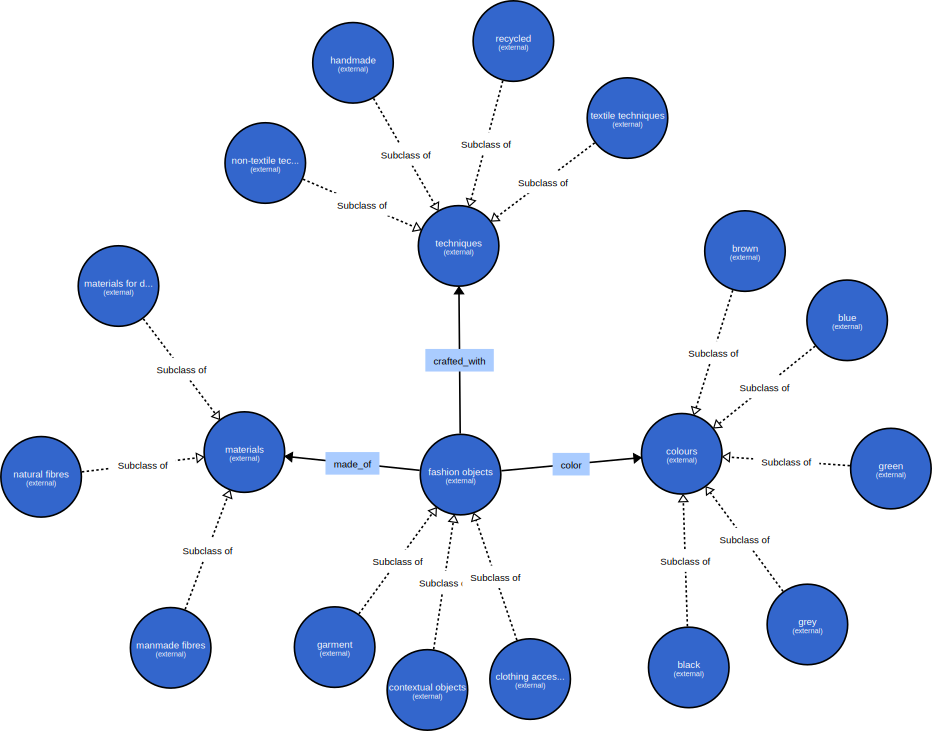
\includegraphics[width=\linewidth]{europeana_relation.pdf}
        \end{figure}
    \end{minipage}
\end{frame}

\begin{frame}{Inferenze in OWL}
	\begin{minipage}{.48\linewidth}
        \begin{block}{Complessità}
            \begin{itemize}
                \item Variazione sintattica di $\mathcal{SROIQ}$
                \item $\mathcal{ALC}$ è una restrizione di $\mathcal{SROIQ}$
                \item $\mathcal{ALC}$ è PSpace-hard
            \end{itemize}
        \end{block}
        \begin{block}{Reasoner}
            \begin{itemize}
                \item Pellet
                \item Fact++
                \item HermiT
                \item \dots
            \end{itemize}
        \end{block}
    \end{minipage}
    \hfill
    \begin{minipage}{.48\linewidth}
        \begin{figure}[h]
            \includegraphics[width=.8\linewidth]{Complexity.pdf}
        \end{figure}
    \end{minipage}
\end{frame}
